\documentclass[border=10mm]{standalone}
\usepackage{tikz}
\usetikzlibrary{arrows, shapes.gates.logic.US, shapes.gates.logic.IEC, calc}

\tikzset{
    my-or-gate/.style={
        or gate US, draw, rotate=0, logic gate inputs=nn
    },
}

\begin{document}

\resizebox{10cm}{!}{

    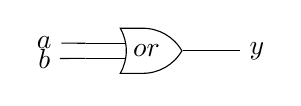
\begin{tikzpicture}[label distance=2mm]

        % INPUTS
        \node[] (A)    at (0,.2)   {\normalsize $a$};
        \node[] (B)    at (0,0)    {\normalsize $b$};

        % OUTPUTS
        \node[] (Y)    at (2.7,.1)  {\normalsize $y$};
        
        % OR, WIRES OR CONNECTOR POINTS
        \node[my-or-gate]   (OR)    at ($(B) + (1.3, .1)$)         {\normalsize $or$};
        \coordinate[]       (ORIN1) at ($(OR.input 1) + (-.5, 0)$) {};
        \coordinate[]       (ORIN2) at ($(OR.input 2) + (-.5, 0)$) {};
        \coordinate[]       (OROUT) at ($(OR.output)  + (.5, 0)$)  {};
        \draw (OR.input 1) -- (ORIN1);
        \draw (OR.input 2) -- (ORIN2);
        \draw (OR.output)  -- (OROUT);

        % INPUT CONNECTIONS
        \draw (A) -- (ORIN1);
        \draw (B) -- (ORIN2);
        
        % OUTPUT CONNECTIONS
        \draw (OROUT) -- (Y);

    \end{tikzpicture}
}

\end{document} 
